\newpage
{\let\cleardoublepage\relax \chapter{Opis działania aplikacji}}
\label{cha:main}



\section{Proces nauczania}
Proces nauczania podzielony jest na 2 etapy :
\begin{itemize}
	\item Trening
	\item Powtórkę
\end{itemize}


\begin{center}
	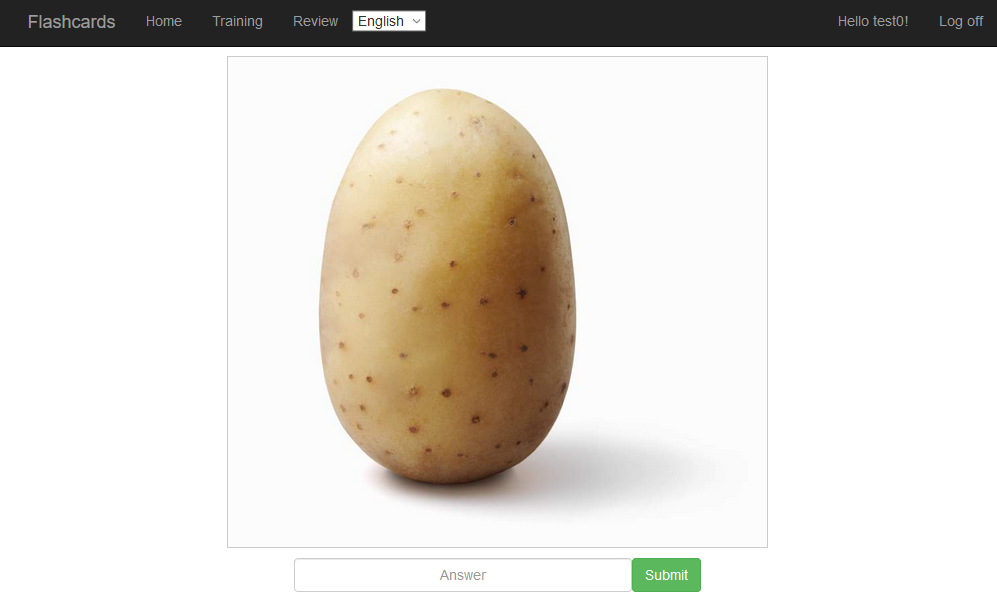
\includegraphics[width=\textwidth]{images/question.png}
	 \captionof{figure}{Widok pytania w projekcie. Jest on wspólny dla każdego z etapów}
\end{center}

\subsection{Trening}

W trakcie treningu użytkownik po raz pierwszy może spotkać się z danym słowem występującym w procesie nauki. Celem tego etapu jest zaznajomienie użytkownika z nowym słowem, zanim zacznie go używać w ramach powtórki.
Trening korzysta z kolejki, wewnątrz której znajduje się maksymalnie 5 fiszek. Tak mała ilość ma na celu łatwiejsze przyswojenie nowego materiału.

W przypadku poprawnej odpowiedzi na pytanie fiszka jest usuwana z kolejki i dodawana do zapamiętanych fiszek, w przeciwnym wypadku przechodzi na koniec kolejki zwiększając ilość niepoprawnych odpowiedzi o 1.

Ilość niepoprawnych odpowiedzi będzie decydować o wskaźniku siły dla danej fiszki po jej wstępnym nauczeniu.

\subsection{Powtórka}

W powtórce mogą wystąpić jedynie te fiszki, na które użytkownik odpowiedział poprawnie w trakcie treningu i ich interwał czasowy od ostatniego powtórzenia już minął. Ten etap także składa się z kolejki, lecz jest ona maksymalnie 30 elementowa. 

W przypadku poprawnej odpowiedzi na pytanie fiszka jest usuwana z kolejki i obliczany dla niej jest nowy interwał oraz siła z jaką jest zapamiętana. W przeciwnym wypadku fiszka jest przesuwana w pewne miejsce kolejki obliczane na podstawie poprzednich niepoprawnych odpowiedzi na tą fiszkę w danej powtórce.

%\subsubsection{Miejsce w kolejce}

%Miejsce w którym fiszka znajduje się po niepoprawnej odpowiedzi jest obliczane tylko na podstawie ilości poprzednich niepoprawnych odpowiedzi i wygląda następująco:
%\begin{minipage}
%\newpage
\begin{center}
\begin{tabular}{| l | l | l |}
\hline
Ilość złych odpowiedzi  & Minimalna pozycja w kolejce & Maksymalna pozycja w kolejce \\ \Xhline{3\arrayrulewidth}

1 & $\frac{1}{3}$ & $\frac{1}{2}$   \\ \hline
2 & $\frac{1}{4}$  & $\frac{1}{3}$   \\ \hline
3 lub więcej & $\frac{1}{5}$   & $\frac{1}{4}$   \\ \hline
\end{tabular}
\captionof{table}{Miejsce w którym znajdzie się fiszka po niepoprawnej odpowiedzi w trybie powtórki}
\label{table:internals}

\end{center}
%\end{minipage}

\begin{center}
	\centering
	\includegraphics[width=\textwidth]{images/interval.png}
	 \captionof{figure}{Zobrazowanie informacji zawartych w tabeli \ref{table:internals}}
\end{center}
%\end{minipage}


\newpage
\subsection{Siła}

Siła jest atrybutem zapamiętanych fiszek dla danego użytkownika. Jest liczbą stałoprzecinkową z zakresu 0-1, gdzie 0 oznacza kompletnie nie zapamiętaną fiszkę, a 1 bardzo dobrze zapamiętaną.  \\
W przypadku poprawnej odpowiedzi na daną fiszkę siła jest obliczana na podstawie poniższych wzorów:  \\

\fbox{
 \addtolength{\linewidth}{-2\fboxsep}%
 \addtolength{\linewidth}{-2\fboxrule}%
 \begin{minipage}{\linewidth}
  \begin{align} \label{eq:winCorr}
   r(x) &= (1 - x^3) * corr \\ 
   \textnormal{Nowa siła} &= \frac{3x + r(x)}{3 + r(x)} \label{eq:winStr}
  \end{align}
 \end{minipage}
}

Gdzie:
\begin{itemize}
	\item x - aktualna ilość siły
	\item corr - Wskaźnik ważności danego tłumaczenia pomnożony przez poprawność wpisanego słowa.
\end{itemize}

\todo[inline]{Mówię o czymś, czego jeszcze nie było}

\begin{center}
	\centering
	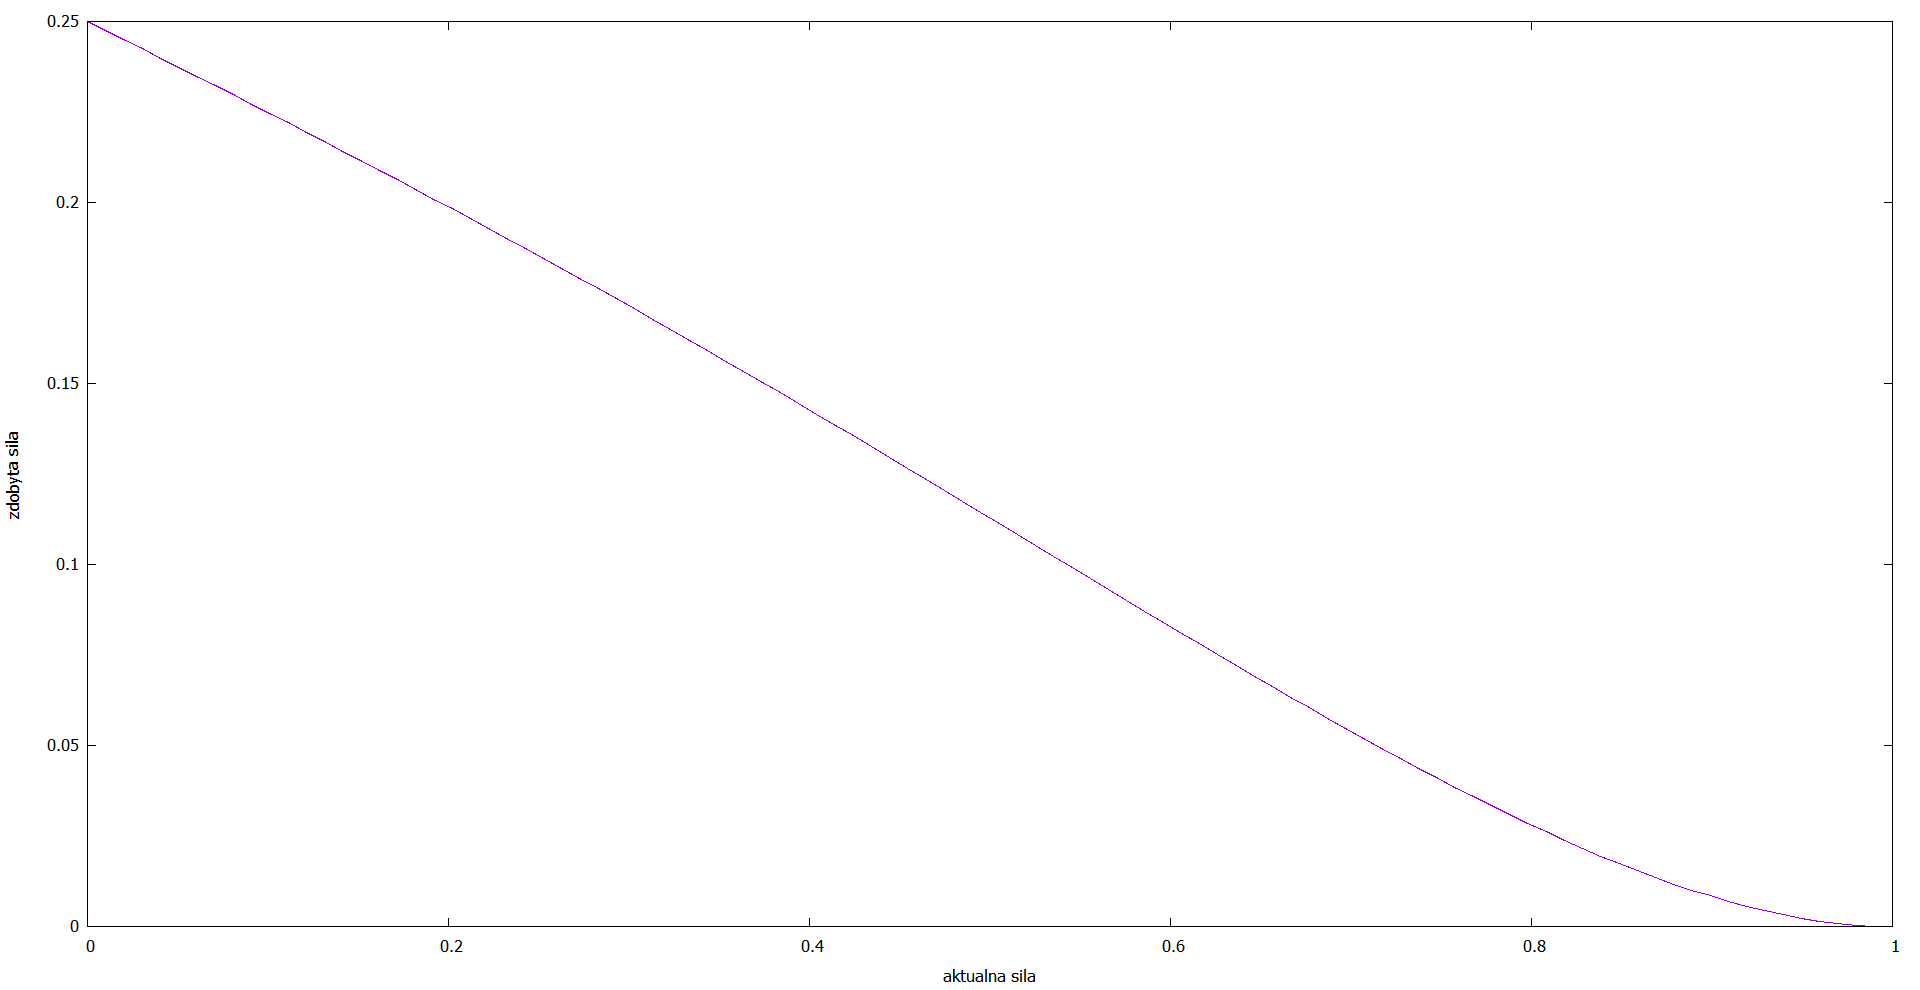
\includegraphics[width=\textwidth]{images/WinStrength.png}
	 \captionof{figure}{Wykres przedstawia ilość zdobytej siły po poprawnej odpowiedzi.}
\end{center}

W przypadku poprawnej odpowiedzi na pytanie, które miało już przynajmniej 1 niepoprawną odpowiedź wzór na nową wartość siły wygląda następująco: \\

\fbox{
 \addtolength{\linewidth}{-2\fboxsep}%
 \addtolength{\linewidth}{-2\fboxrule}%
 \begin{minipage}{\linewidth}
  \begin{equation} \label{eq:lossStr}
  \textnormal{Nowa siła} = \frac{x}{L + x} 
  \end{equation}
 \end{minipage}
}

Gzie L oznacza ilość niepoprawnych odpowiedzi.

\begin{center}
	\centering
	\includegraphics[width=\textwidth]{images/LossStrength.png}
	  \captionof{figure}{Wykres przedstawia ilość straconej siły dla L = 1.}
\end{center}

Wzór na siłę po zakończonym treningu dla danej fiszki wygląda następująco:\\

\fbox{
 \addtolength{\linewidth}{-2\fboxsep}%
 \addtolength{\linewidth}{-2\fboxrule}%
 \begin{minipage}{\linewidth}
  \begin{equation}
  \textnormal{Nowa siła} = \frac{0.5}{L + x} 
  \end{equation}
 \end{minipage}
}

\subsection{Interwały czasowe}

Pomiędzy kolejnymi wystąpieniami danej fiszki w trybie powtórki musi minąć ściśle określony interwał czasowy, który w zależności od poprawności odpowiedzi może maleć lub rosnąć. 
Interwał czasowy zawsze wyrażany jest w dniach. Pierwsze dwa interwały mają odpowiednio wielkość 1 i 6 dni.
\\
W przypadku poprawnej odpowiedzi na dane pytanie nowy interwał jest liczony według następującego wzoru:


\fbox{
 \addtolength{\linewidth}{-2\fboxsep}%
 \addtolength{\linewidth}{-2\fboxrule}%
 \begin{minipage}{\linewidth}
  \begin{align}
  I(n) &= \begin{cases}
  1 & \quad n = 1 \\
  6 & \quad n = 2 \\
  \left \lceil{I(n - 1) * (1 + x * \textnormal{factor})}\right \rceil  & \quad n \geq 3 \\
  \end{cases} \\
  \textnormal{factor} &= 1 - \frac{I(n - 1)}{30}
  \end{align}
 \end{minipage}
}

Gdzie:
\begin{itemize}
	\item I(n) - n-ty interwał
	\item x - Siła obliczona ze wzoru \ref{eq:winStr}
\end{itemize}

W przypadku poprawnej odpowiedzi poprzedzonej serią niepoprawnych odpowiedzi interwał jest liczony według następującego wzoru:


\fbox{
 \addtolength{\linewidth}{-2\fboxsep}%
 \addtolength{\linewidth}{-2\fboxrule}%
 \begin{minipage}{\linewidth}
  \begin{align}
  I(n) &= \left \lfloor{I(n - 1) * \frac{1 - x}{2}}\right \rfloor 
  \end{align}
 \end{minipage}
}

Gdzie x oznacza siłę liczoną według wzoru \ref{eq:lossStr}.

\subsection{Wykrywanie poprawności odpowiedzi}

W celu określenia poprawności odpowiedzi używa się metryki, która w przedziale 0-1 określa podobieństwo dwóch wyrazów. Używana jest w tym celu odległość Levenshteina określająca odległość między dwoma wyrazami na podstawie najmniejszej ilości operacji prostych jakie są potrzebne, aby przekształcić jeden wyraz w drugi. \cite{Leve}

Operacja prosta może być:
\begin{itemize}
	\item Usunięciem danego znaku
	\item Wstawieniem nowego znaku
	\item Zamianą danego znaku na inny
\end{itemize}

W celu uzyskania miary podobieństwa wyrazów używa się poniższego wzoru: 

\fbox{
 \addtolength{\linewidth}{-2\fboxsep}%
 \addtolength{\linewidth}{-2\fboxrule}%
 \begin{minipage}{\linewidth}
  \begin{align} 
  L &= {\frac{|s_1| + |s_2|}{2}}^{1.1} \\
  \textnormal{Podobieństwo} &= \frac{L - D}{L} \label{eq:distance}
  \end{align}
 \end{minipage}
}

Gdzie :
\begin{itemize} 
	\item $s_1$, $s_2$ - wyrazy które porównujemy
	\item D - dystans Levenshteina
\end{itemize}

\vspace{1cm}

Odpowiedź jest poprawna, jeśli:
\begin{itemize}
	\item Ma podobieństwo większe niż 0.82 dla trybu treningowego.
	\item Ma podobieństwo większe niż 0.7 w trakcie powtórki.
\end{itemize}

\subsection{Możliwe odpowiedzi}

Każda fiszka dla danego języka ma zestaw tłumaczeń, które definiują możliwy zbiór poprawnych odpowiedzi. Każde tłumaczenie składa się z:
\begin{itemize}
	\item Poprawnej odpowiedzi.
	\item Zapisu fonetycznego.
	\item Ważności tłumaczenia, która jest używana we wzorze \ref{eq:winCorr}.
\end{itemize}
W trakcie udzielania odpowiedzi na pytanie, wybierane jest to tłumaczenie, które ma największą miarę podobieństwa (\ref{eq:distance}) wśród tłumaczeń dla danej fiszki.

\subsection{Obrazki}

Każda fiszka musi zostać zaopatrzona w odpowiedni zestaw obrazów, z których jeden z nich zostanie wylosowany do procesu sprawdzenia wiedzy użytkownika. Ważne jest, aby obrazki jak najlepiej oddawały przedstawiane słowo i były jak najbardziej zróżnicowane.


\section{Narzędzia administratorskie}

Administrator posiada dodatkowe narzędzia, które pozwalają mu na :
\begin{itemize}
	\item Przeglądanie wszystkich fiszek.
	\item Dodanie nowej fiszki do systemu.
	\item Edycja danej fiszki - dodanie lub edycja tłumaczeń, dodanie lub usunięcie powiązanych obrazków.
\end{itemize}
Prawa administratorskie nadaje się poprzez nadanie roli administratora w tabeli \textbf{AspNetUserRoles}. Aktualnie należy użyć zapytania SQL, aby takowe uprawnienia nadać. 

\begin{center}
	\centering
	\includegraphics[width=\textwidth]{images/Management.png}
	  \captionof{figure}{Widok edycji fiszki.}
\end{center}


\section{Diagramy klas}

Poniżej zostały przedstawione diagramy klas repozytoriów (\ref{section_Repo}), kontrolerów(\ref{section_Kontro}) oraz serwisów, wewnątrz których zdefiniowana jest logika biznesowa aplikacji.

\begin{figure}[h]
	\centering
	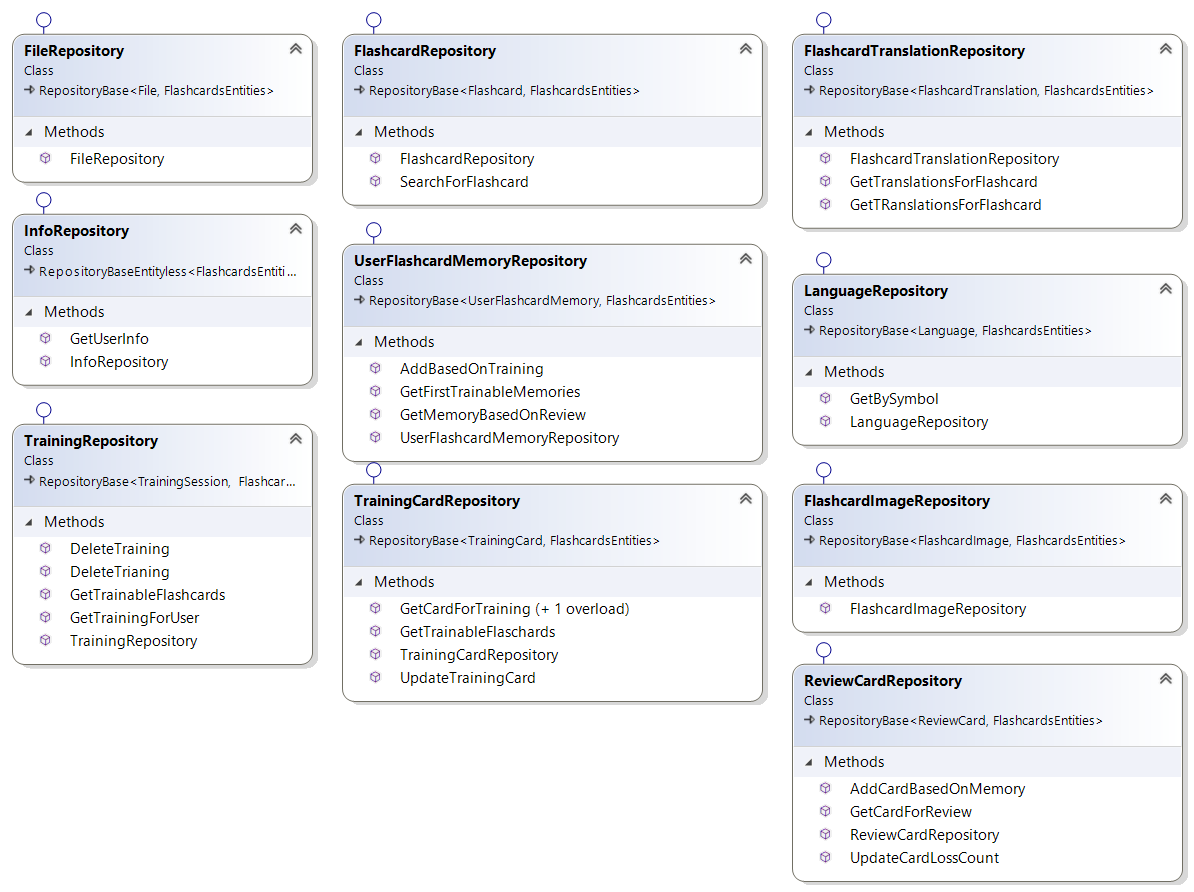
\includegraphics[width=\textwidth]{images/Repos.png}
	 \caption{Diagram klas wszystkich repozytoriów w projekcie wraz z jednostką pracy.}
\end{figure}


\begin{figure}
	\centering
	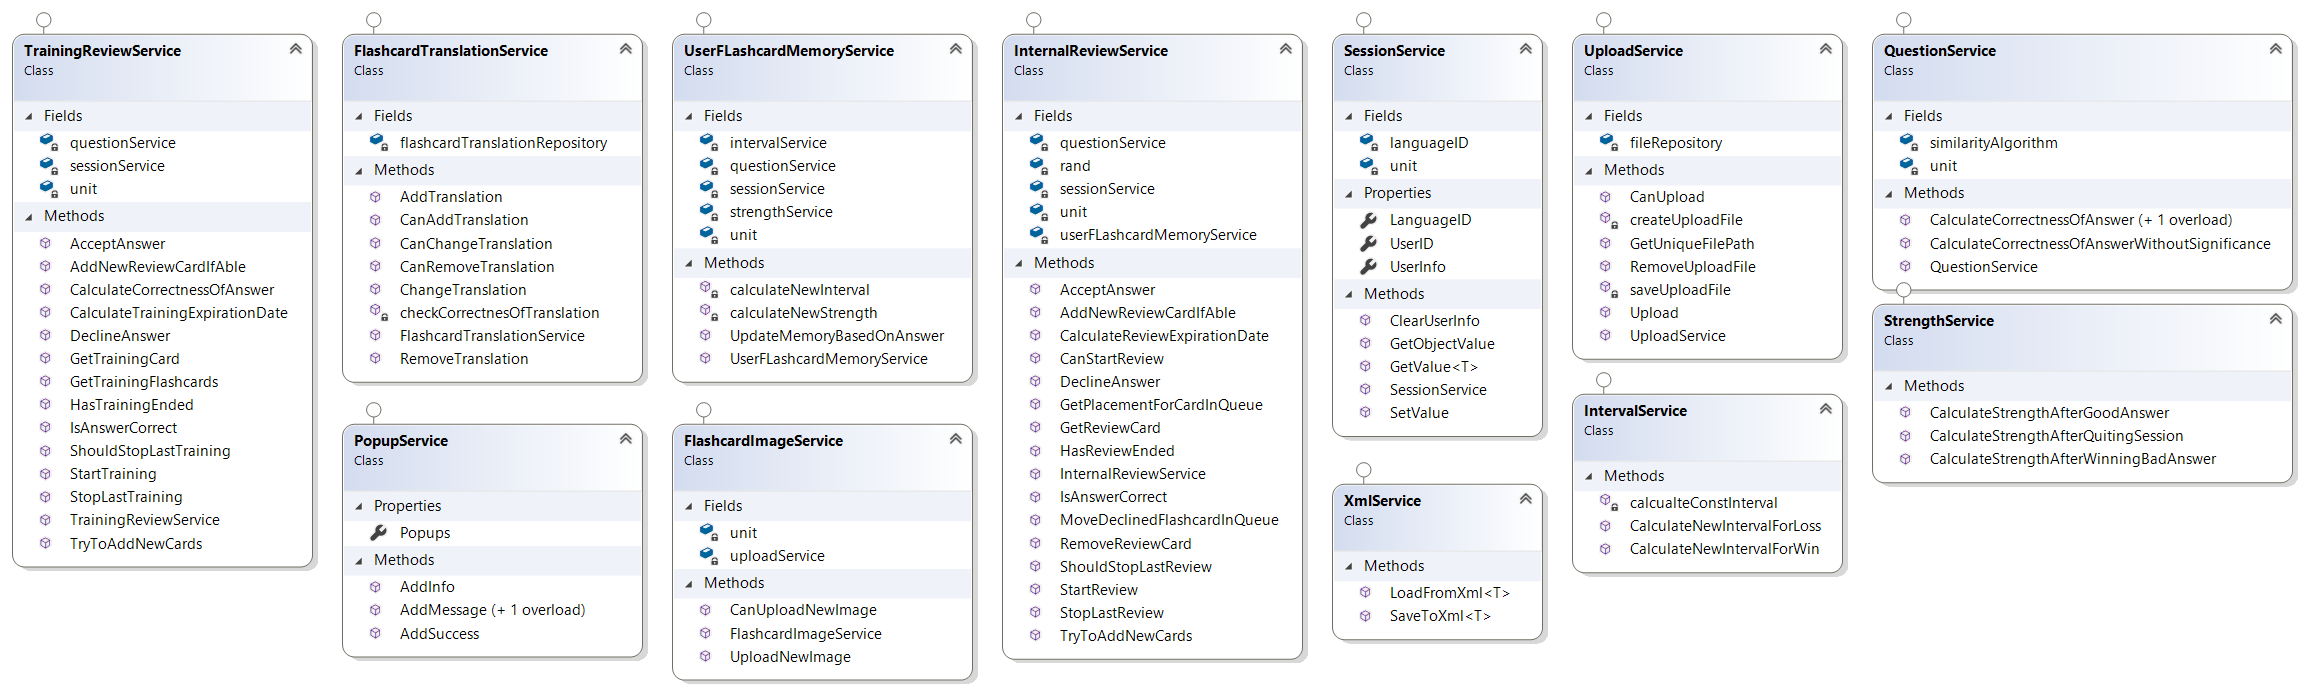
\includegraphics[width=\textwidth]{images/Serwisy.png}
	 \caption{Diagram klas wszystkich serwisów w projekcie}
\end{figure}


\begin{figure}
	\centering
	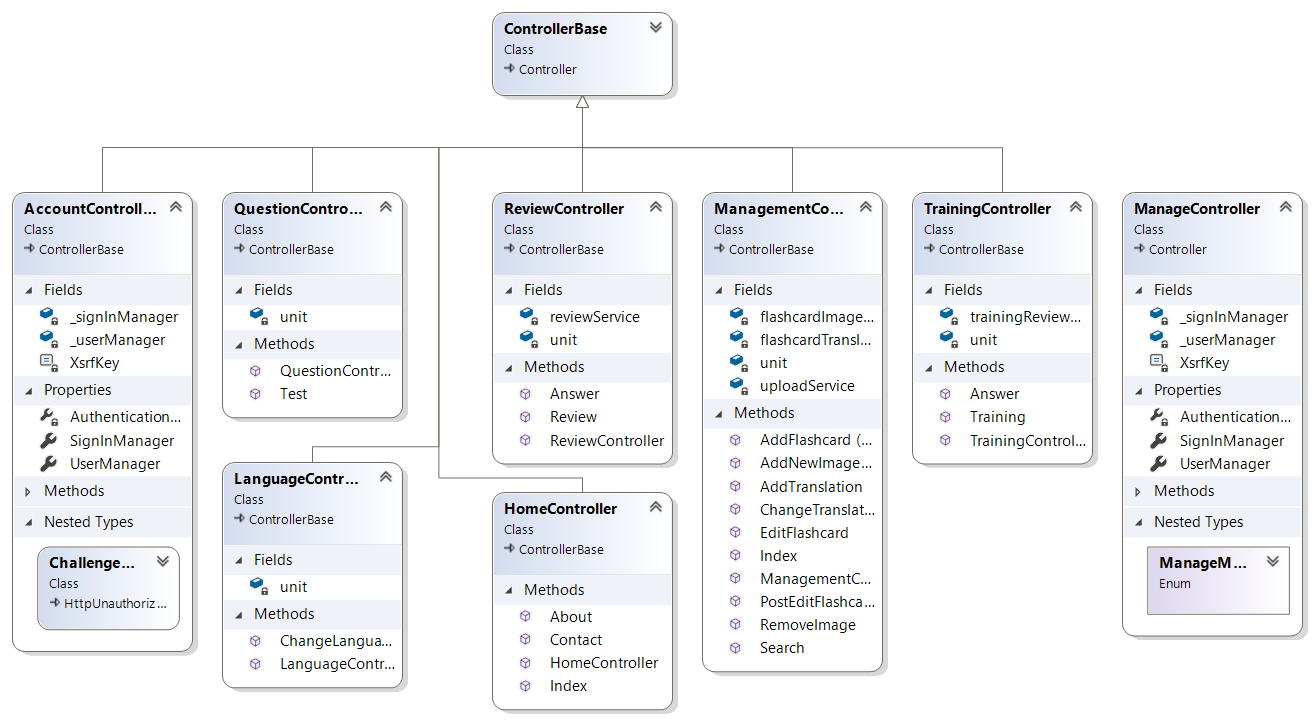
\includegraphics[width=\textwidth]{images/Controllers.png}
	 \caption{Diagram klas wszystkich kontrolerów w projekcie}
\end{figure}


\section{Diagram przypadków użycia}

\begin{center}
	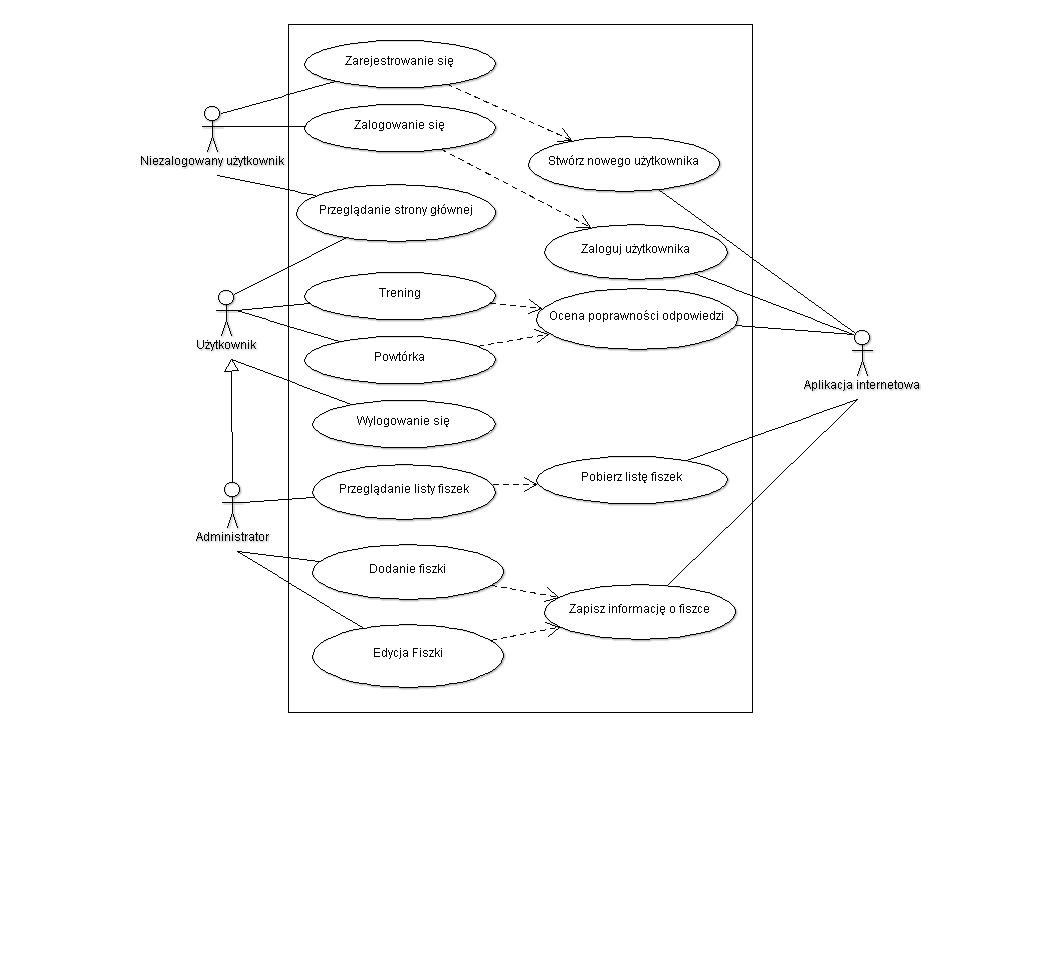
\includegraphics[width=\textwidth]{images/usecases.png}
	 \captionof{figure}{Diagram przypadków użycia.}
\end{center}


\newpage
{\let\cleardoublepage\relax \chapter{Kwestie techniczne}}

\section{Struktura programu}



\section{Przechowywanie danych}

\section{Wyświetlanie stron}

Każdy widok jest tworzony w oparciu o pliki .cshtml, które są wyświetlane przez silnik renderujący Razor. 
